\chapter{Calibration}\label{calibration}

Area Diffraction data can only be analyzed with
a knowledge of how the diffraction experiment was 
set up. Calibration is the process used to find these
values.

\section{The Calibration Algorithm}
    \label{cal_algorithm}\index{calibration}

In principle, all the calibration values could be
measured directly from a diffraction experiment.
In practice, they can not be measured to an 
acceptable level of precision. 
Instead, a calibration procedure is used to 
infer these values from the diffraction data. 
Calibration is done by imaging a calibration standard
before imaging an interesting sample. Assuming 
that the diffraction machine was not altered between the 
imaging of the calibration standard and the 
imaging of the unknown sample, 
the calibration parameters for both sets of data 
will be the same. 
If the calibration values could be determined from
the pattern of the standard crystal, this information 
could be used to analyze the other data.
What it means to use a standard crystal is to know 
in advance its $Q$ values of preferential 
scattering. With these and with the
calibration parameters,
The diffraction pattern that should show up on the detector can
be calculated by, 
for each $Q$ value, varying $\chi$ and calculating the 
corresponding $(x_d,y_d)$ pair. The program can do this. 
If a set of $Q$ values and calibration parameters is enter into 
the program, the \gui{Draw Q Values?} check box 
will draw on top of the diffraction
image what pattern should show up on the detector.
This feature described in section~\ref{displayconstQlines}.

In order to perform the calibration, the calibration parameters 
are varied until they make the calculated pattern match the pattern 
that was captured. The calibration parameters are fit to the 
diffraction pattern. 

\section{Fitting} 
\index{Fitting}\label{fitting_sec}

In order for the fitting algorithm to work, the program 
must already have an initial guess at the calibration 
parameters, a list of the known $Q$ values, and 
a range for each of these $Q$ values. Inside of this 
$Q$ range (as 
calculated by the initial calibration values) there 
must uniquely be the diffraction peak.
An example of this is shown in figure~\ref{divide_up_image}.

\begin{SCfigure}[1][bthp]
    \centering
    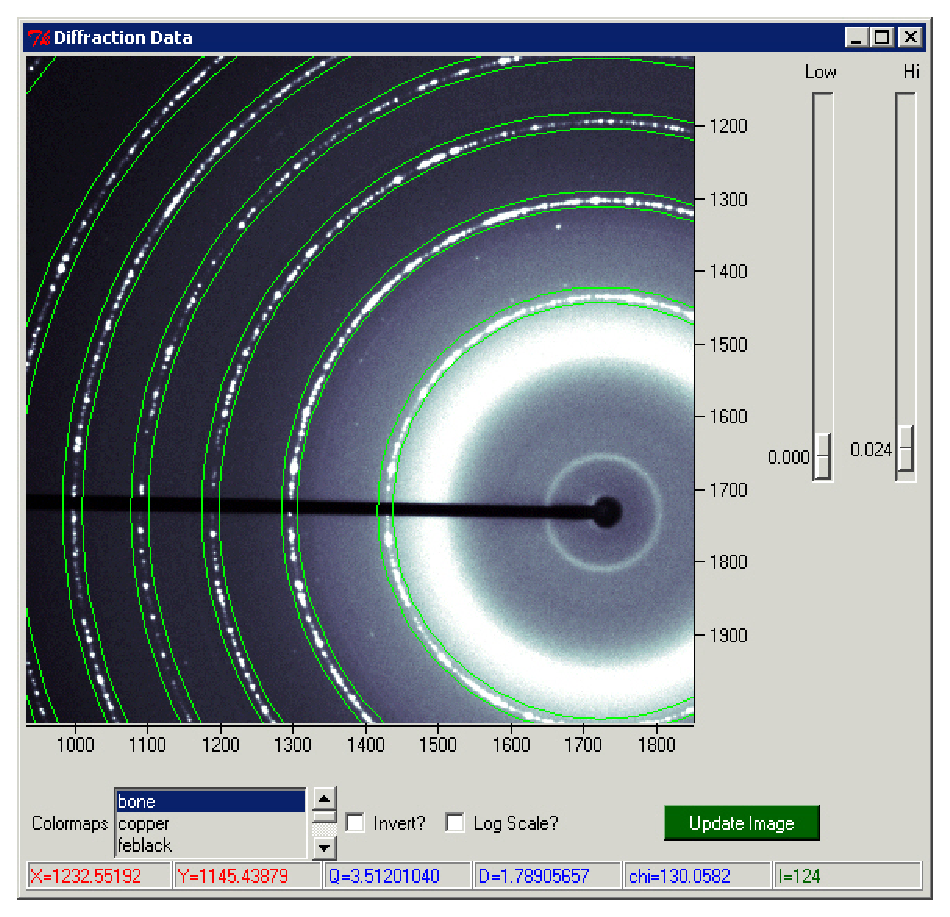
\includegraphics[scale=.75]
    {figures/constant_dq_lines_on_diffraction_image.eps}
    \caption{The diffraction image is divided into
    $Q$ ranges. Each diffraction peak falls
    uniquely into one $Q$ range.}
    \label{divide_up_image}
\end{SCfigure}

\begin{SCfigure}[1][bthp]
    \centering
    % Generated with LaTeXDraw 1.9.3
% Tue Aug 07 18:13:48 PDT 2007
% \usepackage[usenames,dvipsnames]{pstricks}
% \usepackage{epsfig}
% \usepackage{pst-grad} % For gradients
% \usepackage{pst-plot} % For axes
\scalebox{1} % Change this value to rescale the drawing.
{
\begin{pspicture}(0,-4.3)(10.681875,4.3)
\pscircle[linewidth=0.04,dimen=outer](4.3,0.0){1.3}
\pscircle[linewidth=0.04,dimen=outer](4.3,0.0){4.3}
\psline[linewidth=0.04cm](4.4,0.1)(9.4,3.3)
\usefont{T1}{ptm}{m}{n}
\rput(8.548282,4.09){Constant $\chi$ Slice}
\psline[linewidth=0.04cm](4.36,0.48)(4.58,0.02)
\psline[linewidth=0.04cm](5.78,1.38)(6.0,0.92)
\usefont{T1}{ptm}{m}{n}
\rput(6.0514064,0.17){$Q_1$}
\usefont{T1}{ptm}{m}{n}
\rput(4.751406,-0.25){$Q_1-dQ_1$}
\psline[linewidth=0.04cm](7.0,2.12)(7.22,1.66)
\psline[linewidth=0.04cm](8.4,2.96)(8.62,2.5)
\usefont{T1}{ptm}{m}{n}
\rput(6.791406,0.71){$Q_1+dQ_1$}
\usefont{T1}{ptm}{m}{n}
\rput(8.471406,2.05){$Q_2$}
\usefont{T1}{ptm}{m}{n}
\rput(7.751406,1.31){$Q_2-dQ_2$}
\usefont{T1}{ptm}{m}{n}
\rput(9.651406,2.53){$Q_2+dQ_2$}
\psline[linewidth=0.04cm](5.16,0.88)(5.38,0.42)
\psline[linewidth=0.04cm](7.84,2.6)(8.06,2.14)
\pscustom[linewidth=0.04]
{
\newpath
\moveto(4.46,0.3)
\lineto(4.52,0.32)
\curveto(4.55,0.33)(4.6,0.365)(4.62,0.39)
\curveto(4.64,0.415)(4.675,0.45)(4.69,0.46)
\curveto(4.705,0.47)(4.73,0.5)(4.74,0.52)
\curveto(4.75,0.54)(4.775,0.59)(4.79,0.62)
\curveto(4.805,0.65)(4.82,0.715)(4.82,0.75)
\curveto(4.82,0.785)(4.82,0.86)(4.82,0.9)
\curveto(4.82,0.94)(4.835,1.02)(4.85,1.06)
\curveto(4.865,1.1)(4.905,1.16)(4.93,1.18)
\curveto(4.955,1.2)(5.015,1.22)(5.05,1.22)
\curveto(5.085,1.22)(5.16,1.205)(5.2,1.19)
\curveto(5.24,1.175)(5.305,1.15)(5.33,1.14)
\curveto(5.355,1.13)(5.395,1.105)(5.41,1.09)
\curveto(5.425,1.075)(5.455,1.05)(5.47,1.04)
\curveto(5.485,1.03)(5.53,1.02)(5.56,1.02)
\curveto(5.59,1.02)(5.64,1.04)(5.66,1.06)
\curveto(5.68,1.08)(5.73,1.11)(5.76,1.12)
\curveto(5.79,1.13)(5.83,1.15)(5.86,1.18)
}
\pscustom[linewidth=0.04]
{
\newpath
\moveto(7.08,1.92)
\lineto(7.14,1.94)
\curveto(7.17,1.95)(7.22,1.985)(7.24,2.01)
\curveto(7.26,2.035)(7.295,2.07)(7.31,2.08)
\curveto(7.325,2.09)(7.35,2.12)(7.36,2.14)
\curveto(7.37,2.16)(7.395,2.21)(7.41,2.24)
\curveto(7.425,2.27)(7.44,2.335)(7.44,2.37)
\curveto(7.44,2.405)(7.44,2.48)(7.44,2.52)
\curveto(7.44,2.56)(7.455,2.64)(7.47,2.68)
\curveto(7.485,2.72)(7.525,2.78)(7.55,2.8)
\curveto(7.575,2.82)(7.635,2.84)(7.67,2.84)
\curveto(7.705,2.84)(7.78,2.825)(7.82,2.81)
\curveto(7.86,2.795)(7.925,2.77)(7.95,2.76)
\curveto(7.975,2.75)(8.015,2.725)(8.03,2.71)
\curveto(8.045,2.695)(8.075,2.67)(8.09,2.66)
\curveto(8.105,2.65)(8.15,2.64)(8.18,2.64)
\curveto(8.21,2.64)(8.26,2.66)(8.28,2.68)
\curveto(8.3,2.7)(8.35,2.73)(8.38,2.74)
\curveto(8.41,2.75)(8.45,2.77)(8.48,2.8)
}
\end{pspicture} 
}


    \caption{This is a diagram of the peak finding algorithm. 
    The solid black circles represent diffraction peaks. The 
    dotted lines represent the $Q$ ranges. The radial line
    represents the program picking a 
    particular $\chi$ value and looking for peaks along it.
    The program fits a Gaussian to the intensity 
    profile inside each of the ranges to find diffraction 
    peaks.}
    \label{fitting}
\end{SCfigure}

The fitting algorithm first\index{Peak Finding}
finds $(x,y)$ coordinates for many diffraction peaks. 
To do so, it picks a $\chi$ value and 
spread radially out from the center of the diffraction
image. The program makes an array of the intensity
values in each range. It then fits a Gaussian to 
the ranges and the peak of the Gaussian is taken as
the diffraction peak peak. Figure~\ref{fitting} shows
a diagram of this. This is done for many evenly spaced 
$\chi$ values. 
Section~\ref{num_chi_and_stddev} describes how the
number of $\chi$ slices can be set by the user. 

There is not always a consistent diffraction ring 
all the way around the image. Some of the Gaussian fits are
not real peaks and should be ignored. To remove these
spurious peaks, the program applies several tests
to each peak. The first test is that the Gaussian fit was
not too close to the edge of the image. Any peak whose 
fit center plus or minus twice the fit's
standard deviation is outside of the $Q$ range is
considered too close to the edge of the image.
Next, the program tests if the height of the peak 
divided by the standard deviation of the data outside
of the peak is smaller than a certain value. If so,
the peak is not considered to be significant enough.
This value is called \gui{Stddev} and can be specified 
by the user.\index{Stddev} See section \ref{num_chi_and_stddev}.
The higher the value of \gui{Stddev}, the
more picky the program is about allowing peaks. 

After making a list of peaks, the program defines a residual 
function which describes how good the current calibration
parameters are. It converts the $(x,y)$ coordinate
of each peak into a $(Q^{\text{peak}},\chi^{\text{peak}})$ 
pair. Since each peak has a known $Q$ value (which we will 
call $Q^{\text{exp}}$), we define the residual function as
\begin{equation}\label{residual}
    \text{Residual}(x_c,y_c,d,\lambda,\alpha,\beta,R) =  
        \sum_{\text{$x,y$ pairs}}
        (Q^{\text{peak}} - Q^{\text{exp}})^2
\end{equation}
The functional dependence comes from
calculating $Q^{\text{peak}}$ for particular
calibration parameters.
The smaller the residual, the closer the 
calibration parameters are to 
a perfect calibration.

The program takes this function of 7 variables (the
calibration parameters) and minimizes it. 
Ideally, the calibration parameters that minimize the 
residual are the best guess at the calibration parameters.
The program uses the Levenberg-Marquardt nonlinear 
least squares minimization algorithm to minimize the residual. 
The particular implementation used by the program
is Manolis Lourakis's
levmar library\cite{lourakis04LM}. 

\section{Calibrating With the Program}

Calibration is done with the
\gui{Calibration} tab shown 
in figure \ref{calibration_tab} on page
\pageref{calibration_tab}. An image
can be calibrated after a diffraction
image of a standard crystal has been loaded, the $Q$ values for that
crystal have been loaded, and an initial guess 
at the calibration parameters have been loaded.

The \gui{Do Fit}
button can be used to refine the calibration parameters using the 
calibration algorithm described in section~\ref{cal_algorithm}. 
The best guess for the calibration parameters will be put in
the inputs on the \gui{Calibration} tab.

The program will print to the console some useful things
while it does the calibration. The program will calculate the residual 
function (equation \ref{residual}) before and 
after the calibration and print the value to the
console\footnote{Actually, the program
calculates the residual per peak. 
It is a more useful quantity because it is independent
of the number of peaks found.}. The output will look like
\begin{lstlisting}
 - Before fitting, the calculated residual is 5.336138e-04
 - Doing the fitting
 - After fitting, the calculated residual is 6.532131e-06
\end{lstlisting}
The program will display the reason why the fitting
algorithm decided to quit. For example, the program
might print out
\begin{lstlisting}
 - Reason for quitting the fit: 2-stopped by small gradient J^T e
\end{lstlisting}
These reason are told to the program by the fitting
algorithm and they are described on the levmar website
(\url{http://www.ics.forth.gr/~lourakis/levmar/}).
That site says that the different reasons why the
fitting can stop are:
\begin{itemize}
    \item stopped by small gradient J\verb!^!T e
    \item stopped by small Dp
    \item stopped by itmax
    \item start from current p with increased $\backslash$mu
    \item no further error reduction is possible. 
    Restart with increased mu
    \item stopped by small $||$e$||$\_2\cite{lourakis04LM}
\end{itemize}
Stopped by small gradient means that the program found its way
to the bottom of the hill and is convinced that it did its best
job minimizing the function. Stopped by itmax
means that the program was forced to quit by a hard coded limit
on the number of loops through the fitting. The fit should
probably be done again to find the best guess.
I don't know enough about the levmar fitting algorithm to know 
what the other messages really mean. If you need to know, you 
should read the fitting algorithm's documentation. 

The fitting algorithm also displays a covariance matrix that 
it calculates while fitting. I do now know how it calculates this 
and I do not know what it means physically. 
The program print it out after the fitting. 
\begin{lstlisting}[basicstyle=\ttfamily\footnotesize]
Covariance Matrix:
[[ 9.47e-04 -1.76e-04  6.11e-05  3.75e-03  6.37e-06 -3.01e-05  2.45e-02]
 [-1.76e-04  1.24e-03 -1.66e-04 -1.02e-02 -2.58e-05 -5.24e-05 -1.24e-02]
 [ 6.11e-05 -1.66e-04  2.15e-04  1.44e-02  9.19e-06  3.28e-06 -1.52e-03]
 [ 3.75e-03 -1.02e-02  1.44e-02  9.85e-01  5.90e-04  2.10e-04 -1.03e-01]
 [ 6.37e-06 -2.58e-05  9.19e-06  5.90e-04  9.44e-06  1.85e-07 -4.43e-03]
 [-3.01e-05 -5.24e-05  3.28e-06  2.10e-04  1.85e-07  6.70e-06  6.77e-05]
 [ 2.45e-02 -1.24e-02 -1.52e-03 -1.03e-01 -4.43e-03  6.77e-05  4.00e+00]]
\end{lstlisting}
The rows (from top to bottom and from left to right) correspond 
to \gui{xc}, \gui{yc}, \gui{d}
\gui{E}, \gui{alpha}, \gui{beta}, and \gui{rotation}. 
I think that the square root of the diagonal elements of the covariance 
matrix are supposed to correspond to uncertainties, but I do not know 
enough about the minimization algorithm to really be comfortable saying 
that these values are meaningful. The program print out the square root of 
the diagonals. 
\begin{lstlisting}[basicstyle=\ttfamily\footnotesize]
Root of the diagonal of the covariance matrix (I think these are uncertainties)
 - xc         0.0307807389
 - yc         0.0352730417
 - d          0.0146853032
 - E          0.9928960497
 - alpha      0.0030735910
 - beta       0.0025888303
 - R          2.0017867847
\end{lstlisting}
The program can undo to the previous calibration
parameters using the \gui{Previous Values} input.

\section{\texorpdfstring{The \gui{Save Last Fit} 
        Button}{The ``Save Last Fit'' Button}}

Often times, it is desirable to save to a file 
all of the information about a particular calibration
that has been done. Version 2 of the program introduces
a convenient button called \gui{Save Last Fit} that
does just that. After calibrating, pushing this button
and then selecting an output file name will save all of the
information about the previous calibration to a file.
This includes the residual before and after, and the 
covariance matrix, the initial and final calibration
parameters, and the Q list used when calibrating. 
An example is:
\begin{lstlisting}[basicstyle=\ttfamily\footnotesize]
Fit done of: C:/work/LaB6_14_02_56.mar3450

Initial Guess at calibration parameters:
xc      1725.0000000000 0
yc      1725.0000000000 0
D        125.2960000000 0
E      12735.3957721000 0
alpha      0.0000000000 0
beta       0.0000000000 0
R          0.0000000000 0
pl       100.0000000000
ph       100.0000000000

Before fitting, the calculated residual per peak is 0.000533613563184

Refined calibration parameters:
xc      1723.2670576589 0
yc      1729.0275947978 0
D        123.9263391635 0
E      12712.8416444082 0
alpha      0.0043942864 0
beta       0.1124327684 0
R         52.4701069289 0
pl       100.0000000000
ph       100.0000000000

After fitting, the calculated residual per peak is 6.52739855241e-006

Reason for quitting the fit: 2-stopped by small gradient J^T e

Covariance Matrix:
[[ 9.47e-04 -1.76e-04  6.11e-05  3.75e-03  6.37e-06 -3.01e-05  2.45e-02]
 [-1.76e-04  1.24e-03 -1.66e-04 -1.02e-02 -2.58e-05 -5.24e-05 -1.24e-02]
 [ 6.11e-05 -1.66e-04  2.15e-04  1.44e-02  9.19e-06  3.28e-06 -1.52e-03]
 [ 3.75e-03 -1.02e-02  1.44e-02  9.85e-01  5.90e-04  2.10e-04 -1.03e-01]
 [ 6.37e-06 -2.58e-05  9.19e-06  5.90e-04  9.44e-06  1.85e-07 -4.43e-03]
 [-3.01e-05 -5.24e-05  3.28e-06  2.10e-04  1.85e-07  6.70e-06  6.77e-05]
 [ 2.45e-02 -1.24e-02 -1.52e-03 -1.03e-01 -4.43e-03  6.77e-05  4.00e+00]]

Root of the diagonal of the covariance matrix (I think these are uncertainties)
xc         0.0307807389
yc         0.0352730417
d          0.0146853032
E          0.9928960497
alpha      0.0030735910
beta       0.0025888303
R          2.0017867847

Q Data used when calibrating:
             Q           Delta Q
  1.5115438090      0.0500000000
  2.1376468230      0.0500000000
  2.6181029660      0.0500000000
  3.0230876190      0.0500000000
  3.3798737530      0.0500000000
  3.7025252250      0.0500000000
\end{lstlisting}

\section{\texorpdfstring{\gui{Number of Chi?} 
        and \gui{Stddev?}}{``Number of 
        Chi'' and ``Stddev?''}}
        \label{num_chi_and_stddev}

The calibration algorithm requires starting
at the center and moving across the image in constant
$\chi$ slices (see section~\ref{cal_algorithm}).
The number of these slices 
can be set using the \gui{Number Of Chi?} input. 
The default value is 360. 

Section \ref{fitting_sec} describes the \gui{Stddev} parameter.
It can be set using the 
\gui{Stddev?} input. The default value is 5. The higher 
the value, the more likely it is that the program will ignore
bad peaks but the more likely it is that the program
will ignore valid peaks.

\section{\texorpdfstring{Work in 
    $\lambda$}{Work in Lambda}}
    \label{workWavelength}

Often, it is desirable to work with the wavelength 
of the beam instead of its energy. Of course, these
values are related by
\begin{equation}
    E=hc/\lambda.
\end{equation}
The \gui{Work in Lambda} radio select in the menu bar
can be used to work with wavelength in units of nanometers, 
instead of energy, in units of electron volts. 
This can be changed back using the \gui{Work in eV} input.
When the program switches to working with wavelength,
the energy input \gui{E} will be relabeled
\gui{$\lambda$} and the value in the input will be converted.
When working with wavelength, the 
wavelength will be saved to the file instead of the energy when
saving experimental parameters.

\section{Fixing Calibration Parameters}
\label{fix_parameters}

When fitting calibration parameters, it is not
always desirable to allow the program to vary
all of the parameters. For example,
the energy of the beam might be well known already
so it would be desirable to keep it fixed.
The \gui{Fixed?} check boxes next to the parameter
inputs can be used to fix the corresponding parameter
so that it doesn't vary.
The pixel length and pixel height can not be fixed 
because they are never refined. 

\section{\texorpdfstring{Displaying Constant $Q$ 
    Lines}{Displaying Constant Q Lines}}
    \label{displayconstQlines}

After a diffraction file, a list of $Q$ values,
and calibration parameters have been loaded into
the program, the program can display on top of
the diffraction data the diffraction pattern that should
show up for the particular $Q$ lines and the
particular calibration parameters.
This can be done with the \gui{Draw Q Lines?} button on the 
\gui{Calibration} tab. 
Figure~\ref{constant_q_lines_on_diffraction_image}
shows an example. The way that this is done is
described in section~\ref{cal_algorithm}.
Constant $Q$ lines can also be drawn on top of the
caked data. This is described in 
section~\ref{cakeQlinesandpeaks}.  The color of the 
$Q$ lines can be changed using the
\gui{Color} button next to the \gui{Draw Q Lines?} 
button.

\begin{SCfigure}[1][bthp]
    \centering
    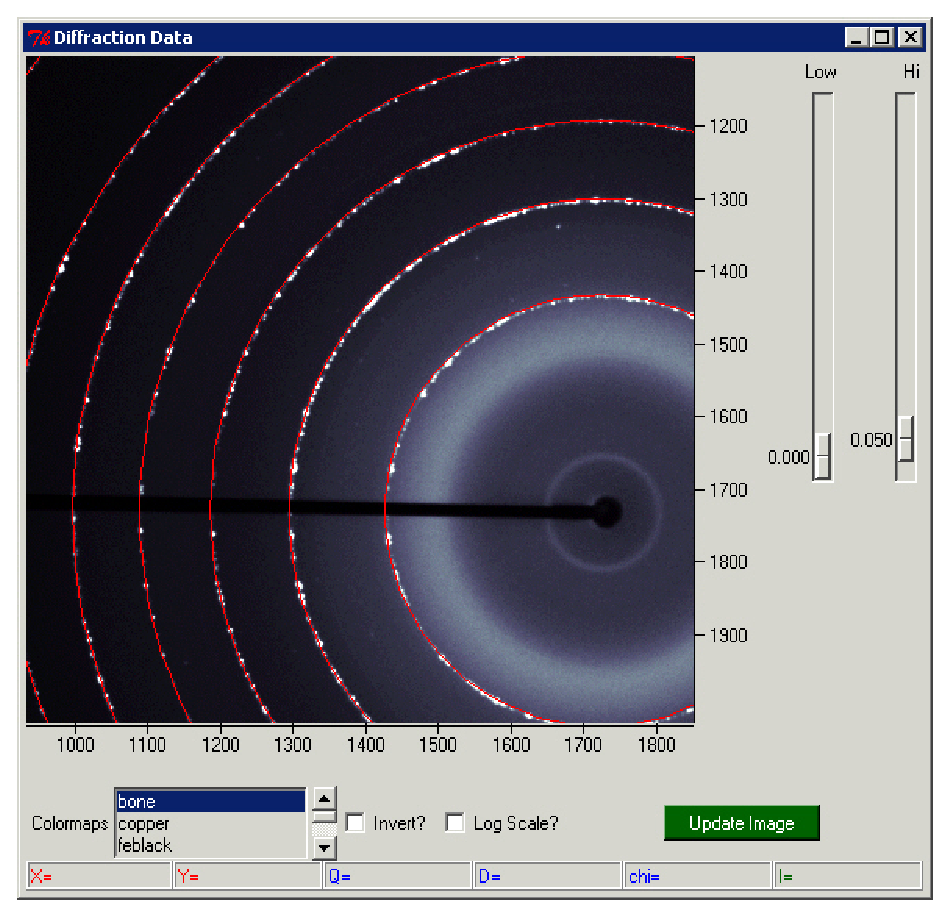
\includegraphics[scale=.75]
        {figures/constant_q_lines_on_diffraction_image.eps}
    \caption{A diffraction image with constant 
    $Q$ lines displayed on it.}
    \label{constant_q_lines_on_diffraction_image}
\end{SCfigure}

\section{\texorpdfstring{Displaying Constant $\Delta Q$ 
    Lines}{Displaying Constant delta Q Lines}}
    \label{displayconstdQlines}

The program can also display on top of the diffraction
data the $Q$ range. The use of this range is 
described in section~\ref{fitting_sec}. 
This can be done with the \gui{Draw dQ Lines?} button.
The color of these lines can be changed with the
corresponding \gui{Color} button. 
Figure~\ref{constant_dq_lines_on_diffraction_image}
shows an example.
Constant $\Delta Q$ lines can also be displayed on top 
of caked data. This is described in 
section~\ref{cakeQlinesandpeaks}.

\begin{SCfigure}[1][bthp]
    \centering
    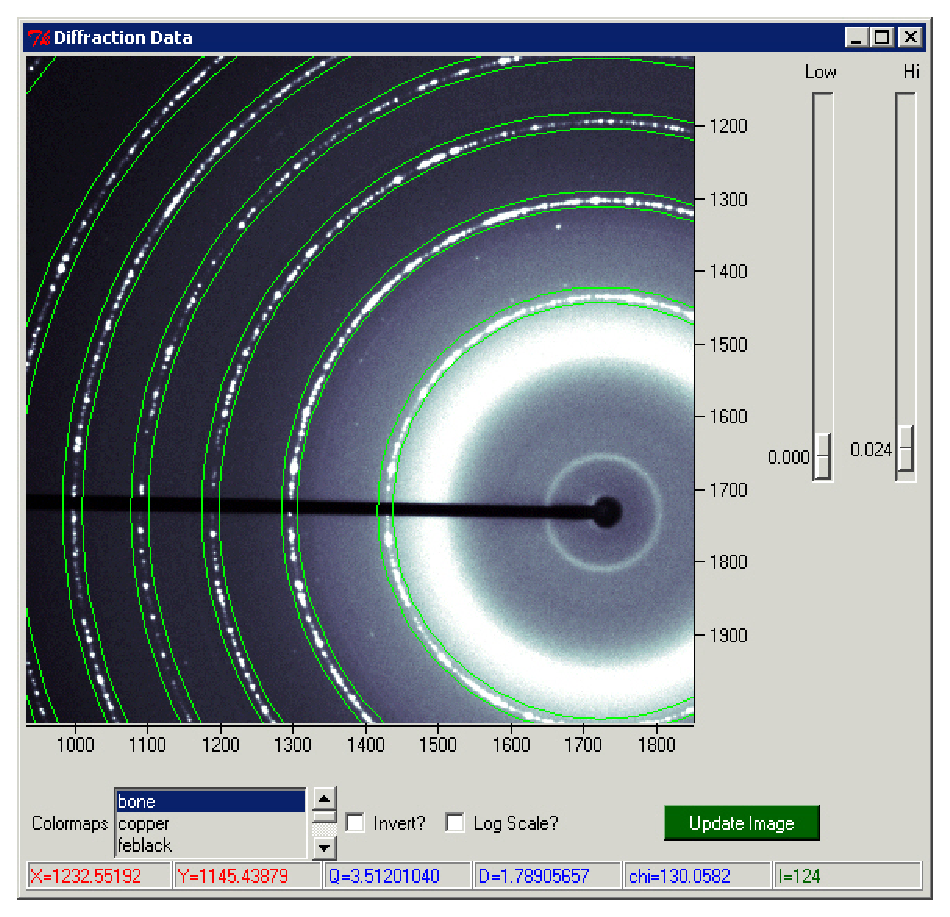
\includegraphics[scale=.75]
    {figures/constant_dq_lines_on_diffraction_image.eps}
    \caption{A diffraction image with the $\Delta Q$ range 
    displayed on it.}
    \label{constant_dq_lines_on_diffraction_image}
\end{SCfigure}

\section{Displaying Peaks}
    \label{displaying_peaks_diffraction}

Section~\ref{fitting_sec} describes how the 
program finds a list of diffraction peaks 
when it performs the image calibration.  
After the program finds the peaks, it can display 
them on top of the diffraction image. 
The \gui{Draw Peaks?} check box can be used to 
display the peaks on the diffraction image as crosses. 
Figure~\ref{peaks_on_diffraction_image} shows 
an example of this. This feature can be used
to see if the program is finding real peaks.
The color of the peaks can be changed with the 
corresponding \gui{Color} button.  
Peaks can also be drawn on top of the caked data. This 
is described in section~\ref{cakeQlinesandpeaks}.

\begin{SCfigure}[1][bthp]
    \centering
    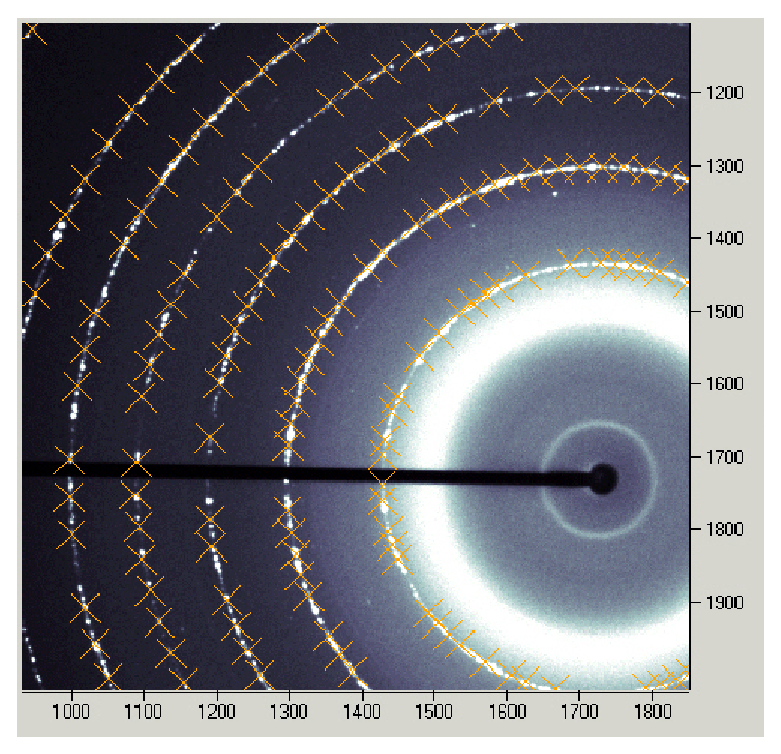
\includegraphics[scale=.75]
    {figures/peaks_on_diffraction_image.eps}
    \caption{A diffraction image with diffraction peaks 
    displayed on it.}
    \label{peaks_on_diffraction_image}
\end{SCfigure}

\section{Masking Peaks}

\begin{figure}[htb]
    \centering
    \subfloat[A diffraction image with diffraction peaks
    and two polygon masks displayed on it.]{
    \label{mask_peaks_diffraction}
    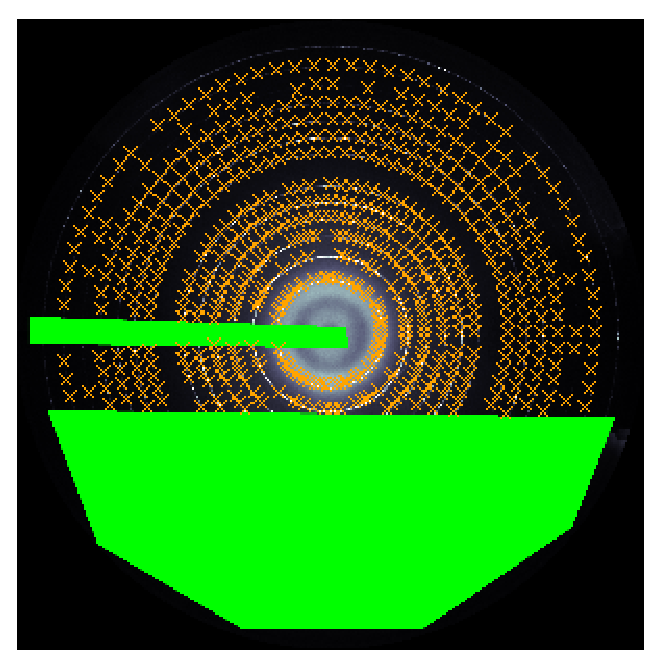
\includegraphics[scale=.7]
    {figures/mask_peaks_diffraction.eps}}\;\;
    \subfloat[A caked plot with diffraction peaks and
    two polygon masks displayed on top of it.]{
    \label{mask_peaks_cake}
    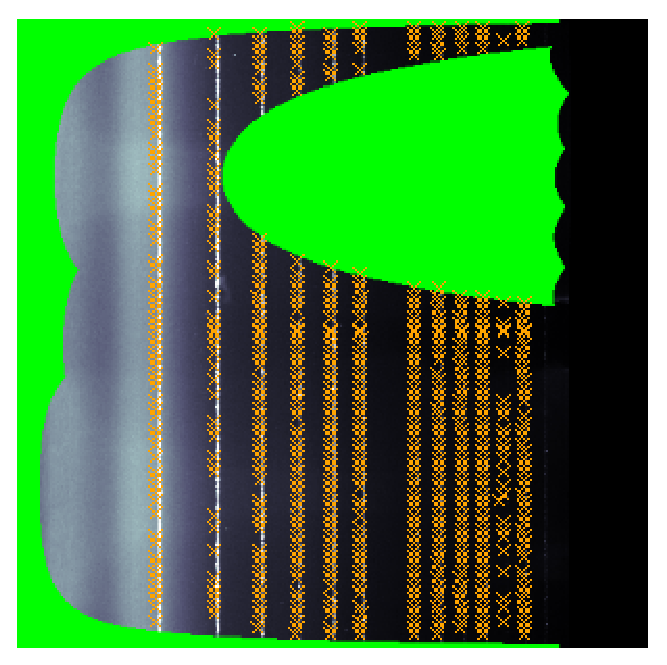
\includegraphics[scale=.7]{figures/mask_peaks_cake.eps}}
    \caption{When a polygon mask is in the program, none
    of the peaks found in the mask will be used while 
    calibrating the image.}
    \label{mask_peaks}
\end{figure}

Polygon masks can be used to stop the program from using peaks 
found in certain regions of the image. See chapter~\ref{pixel_masking} 
for a discussion of masking. No peaks found within polygon masks
will be used when calibrating the diffraction image.
Figure~\ref{mask_peaks_diffraction} shows an example of this. 
Figure~\ref{mask_peaks_cake} shows the same effect on on a caked 
plot. In 
particular, see section~\ref{displaying_peaks_cake} for more 
information on displaying peaks on a caked image. This feature was 
added in version 2.0.0.

\section{Saving the Peak List}

The program can make a list of diffraction peaks and 
save them to a file. If a diffraction image, a list of
standard $Q$ values, and calibration parameters are loaded
in the program, the \gui{Make/Save Peak List} button can
be used to save out the peak list. 
A typical peak list file looks like
\begin{lstlisting}[basicstyle=\ttfamily\footnotesize]
# Diffraction Data: C:/data/LaB6_14_02_56.mar3450
# Calculated on Mon Jun 09 23:41:58 2008
# Calibration data used to find peaks:
#   xc      1723.2670576600 pixels
#   yc      1729.0275948000 pixels
#   D        123.9263391640 mm
#   E      12712.8416444000 eV
#   alpha      0.0043942864 degrees
#   beta       0.1124327684 degrees
#   R         52.4701069289 degrees
#   pl        100.0000000000 microns
#   ph        100.0000000000 microns
# Q data used to find peaks:
# Peaks:
#                Q           Delta Q
#     1.5115438090      0.0500000000
#     2.1376468230      0.0500000000
#     2.6181029660      0.0500000000
#     3.0230876190      0.0500000000
#     3.3798737530      0.0500000000
#     3.7025252250      0.0500000000
#     4.2751481980      0.0500000000
#     4.5346314280      0.0500000000
#     4.7799051400      0.0500000000
#     5.0133130990      0.0500000000
#     5.2360313900      0.0500000000
#     5.4498961800      0.0500000000
#               x                    y               Real Q     ...
  2019.7834513826      1728.4442537319         1.5115438090     ...
  2019.9785942029      1707.6396996094         1.5115438090     ...
\end{lstlisting}
The file contains the calibration parameters
used to generate the peaks and the Q list used
to generate the peaks. Each peak gets its
own line in the file. Each peak is a list of 
space separated numbers.\footnote{In version 1 
of the program, the numbers were tab separated, but
this changed with version 2.} The first two numbers are
the $x$ and $y$ pixel coordinate corresponding of
the peak. The next number is the $Q$ value found in the 
$Q$ list. The next number is the $Q$ value calculated 
at the peak using the calibration
parameters. The next number is the $\chi$ value calculated 
from the pixel coordinate using the calibration parameters. 
The next number is the intensity value at the peak. The final
number is the $2\theta$ value calculated at peak using 
the calibration parameters.

\section{Handling Calibration Data}

There are inputs on the \gui{Calibration} tab 
for the calibration parameters.
\gui{xc} is for the $x$ pixel coordinate of the center of
the image, \gui{yc} is for the $y$ pixel coordinate of
the center of the image, \gui{d} is for the distance from
the sample to the detector,
\gui{E} (or \gui{$\lambda$:}) is for the energy
or wavelength of the beam. The $\alpha$, $\beta$, and
$R$ inputs are for the three rotation angles. 
\gui{pl} is for the pixel length
and \gui{ph} is for the pixel height.
The calibration parameters can be directly entered
using the inputs or they can be loaded and saved 
using the \gui{Load From File} and \gui{Save To File} 
buttons. The format for a calibration data file is 
\begin{lstlisting}
# Calibration Parameters
xc           1725.0000000000 0
yc           1725.0000000000 0
D             125.2960000000 0
E           12735.3957721000 0
alpha           0.0000000000 0
beta            0.0000000000 0
R               0.0000000000 0
pl            100.0000000000
ph            100.0000000000
\end{lstlisting}
Comment lines beginning with
a \# and are ignored. Each of the parameters
is on its own line. Each line is the parameter's 
name followed by spaces or tabs and the
value. The value can be followed by an optional
second number that is whether that parameter
should be fixed or not. 1 means fix the parameter and 0 
means to let it very. If there is no number, the parameter will
not be fixed. $pl$ and $ph$ can not be followed by their fixed value
since they can not be varied.
Instead of energy, the wavelength of the incoming
beam can be stored in a calibration file.
The wavelength line looks like 
\macroline{wavelength	0.973540}.
When the program is in wavelength mode, the program
will wavelength instead of energy as one of the calibration parameters 
The program will load files containing either and do the 
conversion. See section~\ref{workWavelength} for a discussion
of the program working with wavelength instead of energy.


\section{\texorpdfstring{Handling $Q$ Data}{Handling Q Data}}
\label{TheQValues}\index{Q Data}

$Q$ data is loaded into the program with the \gui{Q Data:}
input on the \gui{Calibration} tab. The filename can either 
be entered by hand and then loaded or picked from a file selector 
by pushing the button with the folder icon on it.  Below is an example 
of the $Q$ data file format: 
\begin{lstlisting}
# This is Q Data for Lanthanum Hexaboride
Q   dQ
1.511543809 .05
2.137646823 .05
2.618102966 .05
3.023087619 .05
3.379873753 .05
3.702525225 .05
...
\end{lstlisting}
Comment lines beginning with a \# are ignored. The
first line in the file should be \macroline{Q  dQ} or 
\macroline{Q  delta Q}. The 
rest of the are lines of $Q$ values followed a $\Delta Q$ range.
All $Q$ values must be larger than 0. None of the $Q$ ranges can 
overlap. Instead of $Q$ values, the program can input $D$ values 
If the first line is instead \macroline{D dD} or \macroline{D delta D} the rest of 
the file will be taken to be $D$ and $\Delta D$ values.
The values will be convert using equation~\ref{DtermsQ}. 

\section{\texorpdfstring{The \gui{Standard Q} Menu}{The Standard Q Menu}}

This program stores several common standard $Q$ files as defaults. 
They can be selected through the \gui{Standard Q} option of the 
\gui{Calibration} menu. Selecting one of them will simply put the path
of the $Q$ file into the \gui{Q Data:} input and hit the load for you.
This menu shown on figure~\ref{standard_q_example} on
page \pageref{standard_q_example}. 

You can actually add your own $Q$ data files to this menu by
going into the \gui{StandardQ/} folder inside of the Area
Diffraction Machine's folder and moving your $Q$ data file.
It will show up in the menu the next time you run the program.
It is a little more complicated to do with the Mac distribution
because the whole program is bundled up into one \gui{.app} file.
To do so, you have to right click on the \gui{.app} file, which
is probably in your \gui{Applications/} folder, and select
the \gui{Show Package Contents} option. In the \gui{Contents/}
folder, there is a \gui{Resources/} folder, which contains 
the \gui{StandardQ/} folder where you can put the $Q$ data files.

\section{\texorpdfstring{The \gui{Get From Header?} Input}
    {The ''Get From Header'' Input}}

Sometimes calibration parameters are stored in the header of
a diffraction file.  The \gui{Get From Header} button will 
make the program try to find these values and load them into the 
program.
